\section{Use of \tkzcname{tkzGrid}} \hypertarget{grid}{}

\begin{NewMacroBox}{tkzGrid}{\oarg{local options}\parg{$x_A~;~y_A$}\parg{$x_B~;~y_B$}}%

A few changes for this macro. First of all, to simplify currently the color of
the thinnest grid is determined automatically from the main grid, same process
for the thickness.  This behavior can be modified using styles.

\begin{tabular}{lll}%
options   & default & definition                                        \\
\midrule
\TAline{\parg{$x_A~;~y_A$} \parg{$x_B~;~y_B$}}{(xmin,ymin)(xmax,ymax)} {grid pattern}
\end{tabular}

\begin{tabular}{lll}%
options   & default & definition                                        \\
\midrule
\TOline{sub}{true} {asks for a sub-grid }
\TOline{color}{darkgray}{main grid color}
\TOline{subxstep}{0.2} {the step of the subgraduations for the abscissa axis}
\TOline{subystep}{0.2}{the step of the subgraduations for the ordinate axis}
\TOline{line width}{0.4pt} {main grid line thickness}
\bottomrule
\end{tabular}

\medskip
Default values can be changed in the configuration file or by macros. The color
of the second grid is the same as the main grid, but less intense (by default |gray!50|).
Same behavior for the line thickness (by default |0.75 of linewidth|).
See the examples to change this behavior.
\end{NewMacroBox}

\subsubsection{\tkzcname{tkzGrid} and the option \tkzname{sub}}

The option \tkzname{sub} allows you to display a finer secondary grid.
It is preferable to run \tkzcname{tkzGrid} first, to prevent the grid
from being overlapped with other elements.

\begin{tkzexample}[latex=8cm,small]
\begin{tikzpicture}
  \tkzInit[xmax=4, ymax=2]
  \tkzGrid[sub]
  \tkzAxeXY
\end{tikzpicture}
\end{tkzexample}

\subsubsection{Option \tkzname{sub}}

The option \tkzname{sub} allows to display a finer secondary grid. Some
parameters are modifiable.

\begin{tkzexample}[latex=8cm,small]
\def\tkzCoeffSubColor{20}% instead of 50
\def\tkzCoeffSubLw{0.2}% instead of 0.75
\begin{tikzpicture}
  \tkzInit[xmax=4, ymax=2]
  % we can change the step for the second grid
  \tkzGrid[sub,color=orange,
          subxstep=.5,subystep=.5]
  \tkzAxeXY
\end{tikzpicture}
\end{tkzexample}

\subsubsection{Almost Default}

\begin{tkzexample}[width=8cm,small]
\begin{tikzpicture}
  \tkzInit[xmax=5,ymax=2]
  \tkzGrid[color=orange]
  \tkzAxeXY
\end{tikzpicture}
\end{tkzexample}

\subsubsection{Under the grid, too, option \tkzname{sub}}

\begin{tkzexample}[width=8cm,small]
\begin{tikzpicture}
  \tkzInit[xmax=5,ymax=2]
  \tkzGrid[sub,color=orange]
  \tkzGrid[color=orange]
  \tkzAxeXY
\end{tikzpicture}
\end{tkzexample}

\subsubsection{Grid change}

\begin{tkzexample}[width=8cm,small]
\begin{tikzpicture}
  \tkzInit[xmax=5,ymax=2]
  \tkzGrid[color    = orange,
           sub,
           subxstep = 0.1,
           subystep = 0.1]
  \tkzAxeXY
\end{tikzpicture}
\end{tkzexample}

\subsubsection{Option \tkzname{xstep}, \tkzname{xstep}, \tkzname{subxstep} and \tkzname{subystep}}

\begin{tkzexample}[latex=8cm,small]
\begin{tikzpicture}
  \tkzInit[xmax=.5,xstep=.1,
           ymax=.2,ystep=.1]
  \tkzGrid[sub,
           subxstep = 0.05,
           subystep = 0.05,
           color=orange]
  \tkzAxeXY
\end{tikzpicture}
\end{tkzexample}

\subsubsection{With large intervals}

\begin{tkzexample}[width=8cm,small]
\begin{tikzpicture}
  \tkzInit[xmax=100,xstep=20,
           ymax=3000,ystep=1000]
  \tkzGrid[sub,subxstep=10,
               subystep=500,
               color=orange]
  \tkzAxeXY
\end{tikzpicture}
\end{tkzexample}

\subsubsection{\tkzcname{tkzGrid} and the arguments}

The grid can be any size.

\begin{tkzexample}[width=8cm,small]
\begin{tikzpicture}
  \tkzInit[xmax=100,xstep=20,
           ymax=3000,ystep=1000]
  \tkzGrid[sub,subxstep=10,
           subystep=500,
           color=orange]
           (-20,-1000)(115,4000)%
  \tkzAxeXY
\end{tikzpicture}
\end{tkzexample}

\subsubsection{Use of \tkzname{pi} with \tkzcname{tkzGrid}}

\begin{tkzexample}[width=8cm,small]
\begin{tikzpicture}[scale=.75]
  \tkzInit[xmax=6.5,ymax=6.5]
  \tkzGrid[xstep=pi,ystep=pi/2,sub,
           subxstep=pi/4,subystep=pi/4]
  \tkzLabelX[label=$t$,orig=false,trig=4,
           below=6pt,font=\scriptsize]
  \tkzLabelY[trig=2,font=\scriptsize]
  \tkzDrawXY
\end{tikzpicture}
\end{tkzexample}

\subsubsection{Options \tkzname{frac} and \tkzname{trig} with \tkzcname{tkzGrid}}

\begin{tkzexample}[width=8cm,small]
\begin{tikzpicture}
  \tkzInit[xmax=9,xstep=3,ymax=4]
  \tkzGrid[xstep=1,ystep=pi/2,sub,
           subxstep=1,subystep=pi/4]
  \tkzLabelX[label=$t$,orig=false,frac=3,
           below=6pt,font=\scriptsize]
  \tkzLabelY[trig=2,font=\scriptsize]
\end{tikzpicture}
\end{tkzexample}

\subsubsection{Use of a repetition grid}

\begin{tkzexample}[latex=8cm,small]
\begin{tikzpicture}[scale=.5]
  \tikzset{xaxe style/.style ={-}}
  \tkzInit[xmax=15,ymax=15]
  \tkzClip
  \tkzGrid[sub,color=orange]
  \tkzLabelX[label= ]   \tkzLabelY[label= ]
  \tkzDrawXY
  \node[opacity=.5] at (8,6){%
    
\includegraphics[scale=.5]{tiger}};
\end{tikzpicture}
\end{tkzexample}

\endinput
